\documentclass{article}
\usepackage[utf8]{inputenc}
\usepackage[margin=1in]{geometry} % set margins
\usepackage{listings} % for code
\usepackage{graphicx} % for images
\graphicspath{ {./images/} } % path for images
\usepackage[linewidth=1pt]{mdframed} % for making boxes
\usepackage[shortlabels]{enumitem} % provides control over enumerate, itemize, and description
\usepackage{colortbl} % for coloring cells
\usepackage{tabularx} % for tables spanning textwidth
\usepackage{pifont} % for xmark and cmark
\usepackage{multirow} % for multirow in tables
\usepackage{longtable} % for person covariates table
\usepackage{booktabs} % for toprule and midrule
\usepackage{setspace} % for double spacing
\newcommand{\cmark}{\ding{51}}%
\newcommand{\xmark}{\ding{55}}%

% For tables
\usepackage{float} % control over floating tables
\usepackage{array} % fixed table width
\newcolumntype{P}[1]{>{\centering\arraybackslash}p{#1}} % define a new column type with horizontal centering
\renewcommand{\arraystretch}{1.3} % adjust linespace between tables

% Style for listings
\lstset{
basicstyle=\small\ttfamily,
columns=flexible,
breaklines=true
}

% Use biblatex
\usepackage[style=authoryear, giveninits=true]{biblatex} % display author (only initials) and year in citations
\addbibresource{final-references.bib} % use this bib file
\DeclareNameAlias{sortname}{last-first} % display last name first
\DeclareFieldFormat{url}{Available at\addcolon\space\url{#1}} % change url to available at
% break long urls in biblatex
\setcounter{biburllcpenalty}{7000}
\setcounter{biburlucpenalty}{8000}

% Spacing
\setlength{\parindent}{0pt}
\doublespacing % set double spacing

\begin{document}

\title{Effect of Instrument, Harmonic Motion, and Voice Leading on Classical Music Classification}
\author{Myung Kyung (Rachel) Hyeon \footnote{Department of Statistics \& Data Science, Carnegie Mellon University} \\\texttt{mhyeon@andrew.cmu.edu}}
\date{December 11, 2022}

\maketitle

% Abstract might need to add one or two sentences about what methods are used in this paper.

% Good abstract. Maybe try to make sure that the abstract addresses all parts of the IDMRAD. But I like how you discuss the main result of the research questions. Good job.

\begin{abstract}
    This paper analyzed data collected by Ivan Jimenez, a composer and musicologist visiting the University of Pittsburgh, and student Vincent Rossi, for a study measuring the influence of instrument, harmonic motion, and voice leading on listeners' identification of musical stimuli as ``classical'' or ``popular''. Two research questions were investigated in this paper: (1) what experimental factor, or combinations of factors, has the strongest influence on rating a music as ``classical'', and (2) if there are differences in the way that musicians and non-musicians identify classical music. The raw data used for analysis contained 2520 observations and 28 variables, but only 1540 observations were complete. To answer the first research question, a final linear model was selected after performing model selection using information criteria, Analysis of Variance test, and backward selection of fixed effects. To answer the second research question, participants were dichotomized into two groups, musicians and non-musicians, and the interactions between the dichotomized variable and other predictors were assessed. It was found that listeners think piano and especially strings, sound more classical than guitar, the harmony I-V-VI have a strongest association with classical ratings among the four levels of harmonic motion, and contrary motion have the strongest association with classical ratings among the levels of voice leading. Also, musicians tend to rate harmony structure I-V-VI as classical differently from how non-musicians rate them. Limitations of the study include a large amount of missing data and a potential small sample bias affecting some coefficient estimates of the final linear model.
\end{abstract}



\section{Introduction}

%I would suggest using a broad background to introduce this and put the current version in the Data section so that the introduction and data section don't get repetitive.

% Really good introduction. I really like the way you lay out your 2 research questions and address the sub-questions within the first research question. I wonder whether the discussion of the factors within the stimuli and the response variables should be included here or in the data section. it makes sense to me the way you did it, but something to think about. Good job.

Although classical music is not limited to a single definition, classical music generally refers to a form of formal European music of the late 18th to early 19th century \parencite[]{oxford-dict}. Classical music is characterized by ``harmony, balance, and adherence to established forms'' \parencite[]{oxford-dict}. On the other hand, popular music generally refers to a form of music that has a wide appeal to a general audience, and is characterized by ``lightly romantic or sentimental melodies'' \parencite[]{collins-dict}. An example of a study that studied what factor differentiates classical music from popular music is a study conducted by De Clercq and Temperley \parencite*{declercq-2011} where the researchers found that popular music from five decades (50s to 90s) had different distribution of chromatic roots than classical music from the 18th to 19th century. Many studies were conducted on assessing listeners' ability to identify music based on song characteristics. Doll \parencite*{doll-2017} found that common chord progressions found in North American and British popular music can be stored in the long-term memories of listeners and be recognized as ``stereotypical''. Listeners were able to identify a piece of music based on the pitch and rhythmic features of the melody even when melody was presented in a different instrument or tempo \parencite[]{warren-1991, andrews-1998, dowling-2008}. A study by Jimenez and Kuusi \parencite*{Jimenez-2018} found that listeners were able to identify music from chord progressions, and musicians performed better than non-musicians at this task. The motivation for this study is to examine the influence of three design variables, Harmony, Instrument, and Voice on listeners' classification of music as classical.

\bigbreak

In this paper, we will analyze the data collected by Ivan Jimenez, a composer and musicologist visiting the University of Pittsburgh, and student Vincent Rossi, for a study measuring the influence of instrument, harmonic motion, and voice leading on listeners' identification of a series of three-chord successions as ``classical'' or ``popular'' \parencite{Jimenez-presentation}. The researchers presented 36 musical stimuli to 70 listeners, recruited from the population of undergraduates at the University of Pittsburgh \parencite{homework-9}. Listeners were asked to rate the musical stimuli on a scale of 1 to 10 on how classical and how popular the music sounds, with 1 being not at all, and 10 being very classical or very popular. Listeners were told that a piece could be rated as both classical and popular, neither classical nor popular, or mostly classical and not popular (or vice versa), so that the scales should have functioned more or less independently.

\bigbreak

The 36 stimuli were chosen by completely crossing these factors:
\begin{itemize}
    \item Instrument: String Quartet, Piano, Electric Guitar
    \item Harmonic Motion: I-V-VI, I-VI-V, I-V-IV, IV-I-V
    \item Voice Leading: Contrary Motion, Parallel 3rds, Parallel 5ths
\end{itemize}

This paper will address the following research questions:

\begin{enumerate}
    \item What experimental factor, or combinations of factors, has the strongest influence on ratings?
    \begin{enumerate}
        \item Does Instrument exert the strongest influence among the three design factors (Instrument, Harmonic Motion, Voice Leading), as the researchers suspect?
        \item Among the levels of Harmonic Motion does I-V-VI have a strong association (the strongest) with classical ratings? Does it seem to matter whether the respondent is familiar with one or the other (or both) of the Pachelbel rants/comedy bits?
        \item Among the levels of Voice Leading, does contrary motion have a strong (the strongest) association with classical ratings?
    \end{enumerate}
    \item Are there differences in the way that musicians and non-musicians identify classical music?
\end{enumerate}



\section{Data}

% If you had to change the raw data in any way (e.g. deleting cases or variables, performing imputation, correcting mistyped data, deleting cases with crazy data, etc.), please describe what you did and provide justifications, as part of the Data section.

% It may also be the case that you used different versions of the data set for different questions. Please describe and justify this in the Data section too, if you did so.

% TBD, the data section needs more work to do. I think you are on the right track. You mentioned you clean the data, and I would like to see some footnotes to remind me to look at the appendix. Some notes for future work is that you may want to introduce the variables in the data set and some EDA plot which you can do deeper analysis in the result section.

% Great data section. I like how you discuss the way that you broke up and subsetted the dataset in your analysis. I also like how in depth you go about where the data is being extracted from. Going back to my previous point about the stimuli in the intro, you do a good job not being redundant with that information, so I suppose just think about whether the factors of the stimuli should stay where it is or moved to this section. Overall, awesome section.

% SPLIT UP THE APPENDIX A (replace Appendix A.1!!!!!!) with smaller sections of the appendix

The raw data provided by Dr. Jimenez consisted of 2520 observations of 28 variable each, fully balanced across 70 listeners/subjects and 36 experimental conditions (Appendix A.1). The data has two levels: level-1 observations are ratings of how Classical each musical stimulus sounds, and level-2 groups are the set of stimuli that each listener rated. A brief description of all variables in the data set is presented in Table \ref{table:vardef}.

\bigbreak

From the raw data, we created two data sets for the analysis:
\begin{itemize}
\item \texttt{fulldata} is a data set consisting of all of the original variables except for \texttt{X1stInstr}, \texttt{X2ndInstr}. \texttt{X1stInstr} and \texttt{X2ndInstr} were removed because 87\% of \texttt{X2ndInstr} column and 60\% of \texttt{X1stInstr} column were missing data (Appendix A.3). 27 rows from \texttt{fulldata} that had missing Classical and Popular response values were also removed (Appendix A.4). Furthermore, two responses of 19 for Classical and Popular ratings were deleted as 19's were assumed to be keying errors when entering the data (Appendix A.2). After deletion, this data set has 2491 observations of 26 variables, and is nearly balanced across the 70 subjects and 36 experimental conditions (Appendix A.4). With the \texttt{fulldata} data set, I explored the influence of the three experimental factors, both fixed and random effects, on Classical ratings.
\item \texttt{nomissdata} is a subset of \texttt{fulldata} with no missing values. This data set has 1540 complete observations of 26 variables.  It is reasonably well balanced across experimental conditions and subjects, but represents only 43 of the original 70 subjects (Appendix A.4). With the \texttt{nomissdata} data set, we did variable selection on the person covariate fixed effects and re-considered random effects in light of a final person covariates model.
\end{itemize}

The distributions of the variables in \texttt{fulldata} and \texttt{nomissdata} are similar (Appendix A.5).  Although three quantitative variables (\texttt{OMSI}, \texttt{X16.minus.17}, and \texttt{NoClass}) exhibit noticable skewing, no transformations were conducted to make the results as immediately interpretable.

\begin{table}
\caption{Description of 28 variables in the data set.\label{table:vardef}}
\ttfamily
\bigbreak
\begin{tabular}{| P{5cm} | m{10.8cm} |}
\hline
\textbf{Variable} & \textbf{Variable Definition} \\
\hline\hline
X & Line number in the data set (IGNORE.) \\
\hline
Classical & How classical does the stimulus sound? \\
\hline
Popular & How popular does the stimulus sound? \\
\hline
Subject & Unique subject ID \\
\hline
Harmony & Harmonic Motion (4 levels) \\
\hline
Instrument & Instrument (3 levels) \\
\hline
Voice & Voice Leading (3 levels) \\
\hline
Selfdeclare & Are you a musician? (1-6, 1=not at all) \\
\hline
OMSI & Score on a test of musical knowledge \\
\hline
X16.minus.17 & Auxiliary measure of listener’s ability to distinguish classical vs popular music \\
\hline
ConsInstr & How much did you concentrate on the instrument while listening (0-5, 0=not at all) \\
\hline
ConsNotes & How much did you concentrate on the notes while listening? (0-5, 0=not at all) \\
\hline
Instr.minus.Notes & Difference between prev. two variable \\
\hline
PachListen & How familiar are you with Pachelbel’s Canon in D (0-5, 0=not at all) \\
\hline
ClsListen & How much do you listen to classical music? (0-5, 0=not at all) \\
\hline
KnowRob & Have you heard Rob Paravonian’s Pachelbel Rant (0-5, 0=not at all) \\
\hline
KnowAxis & Have you heard Axis of Evil’s Comedy bit on the 4 Pachelbel chords in popular music? (0-5, 0=not at all) \\
\hline
X1990s2000s & How much do you listen to pop and rock from the 90’s and 2000’s? (0-5, 0=not at all) \\
\hline
X1990s2000s.minus.1960s1970s & Difference between prev variable and a similar variable referring to 60’s and 70’s pop and rock. \\
\hline
CollegeMusic & Have you taken music classes in college (0=no, 1=yes) \\
\hline
NoClass & How many music classes have you taken? \\
\hline
APTheory & Did you take AP Music Theory class in High School (0=no, 1=yes) \\
\hline
Composing & Have you done any music composing (0-5, 0=not at all) \\
\hline
PianoPlay & Do you play piano (0-5, 0=not at all) \\
\hline
GuitarPlay & Do you play guitar (0-5, 0=not at all) \\
\hline
X1stInstr & How proficient are you at your first musical instrument (0-5, 0=not at all) \\
\hline
X2ndInstr & Same, for second musical instrument \\
\hline
first12 & In the experiment, which instrument was presented to the subject in the first 12 stimuli? (IGNORE.) \\
\hline

\end{tabular}
\end{table}


\section{Methods}

% Well done! I really like that you named the full name of AIC, BIC, DIC, and cAIC. That makes me know what you are doing and using. You explained the methods you use in different sections in the results section which is also really clear. I think you also use some other methods like fitLMER function in R but you didn't mention it in the method. Reread your results and appendix section to see what are some missing methods. From now, I can tell that you are missing fitLMER function and regression part.

% I like how you mention all of the pertinent metrics that you will be using from your technical appendix to evaluate your findings. I also like how the methods are targeted in how each method is helping to answer the research questions and what part of it. I suggest using sub headings in this section, it makes parsing through and scanning the section a lot easier to read and quicker for reference when looking back later on in the paper. Once again, great job.

% Cite R and R studio

All statistical analyses were conducted using R \parencite{r}. 

\subsection{Statistical Analysis for First Research Question}

To answer the first research question, ``What experimental factor, or combinations of factors, has the strongest influence on ratings?'', we developed a final model that accurately models the relationship between Classical ratings and various experimental factors. Model selection was conducted in four steps, which are listed below. The intermediate model that was selected in the previous step was used as a basis when deciding to add more experimental factors in the next step. Both the intermediate models and the final model that was selected will be presented. The final model obtained after completing step 4 will be used to answer the first research question.
\bigbreak

Model selection steps:
\begin{enumerate}
    \item Testing whether interaction term(s) between three design variables (\texttt{Harmony}, \texttt{Instrument}, \texttt{Voice}) are needed
    \item Testing whether including the random intercept is preferred by information criteria and ANOVA test
    \item Testing whether adding random slope(s) is/are preferred by information criteria
    \item Selecting fixed effects (person covariates) to include in the model using backward selection
\end{enumerate}

During the model selection process, Analysis of Variance (ANOVA) test and three information criterions (Akaike information criterion (AIC), Bayesian information criterion (BIC), and Deviance information criterion (DIC)), and backward selection of person covariates were used. Analysis of Variance (ANOVA) test between regression models were performed using the \texttt{anova()} function in R to compare between the nested models with differing interactions and random effects \parencite{r}. The \texttt{anova()} function performs a Chi-square test between a reduced model and a full model where the reduced model is nested within a full model to test the null hypothesis that the coefficients are zero for all variables in the full model that are not in the reduced model \parencite{stack-1}. The alternative hypothesis is that the coefficients for all variables in the full model that are not in the reduced model are not zero. In this paper, we used a significance threshold of 0.05. AIC, BIC, and DIC are information criteria that are used for model selection. AIC, BIC, and DIC all use a model's maximum likelihood estimation (log-likelihood) as a measure of fit, but each of the three information criteria differ in what aspects of the model it penalizes. AIC tends to pick larger models with lower prediction error \parencite[]{lecture-22}. BIC tends to pick simpler models that are closer to the true model \parencite[]{lecture-22}. DIC is a generalization of AIC where it can compute score for hierarchical models. DIC is designed to correctly count degrees of freedom when comparing models with random effects. Therefore, DIC of a linear regression model is the same as AIC of the same linear regression model \parencite[]{lecture-22}. For all three information criteria, a model with smaller information criterion score compared to another model means that the model with smaller score is a preferred model. After identifying which combinations of interaction between three design variables and what random effects should be added, person covariates were added to the final model after variable selection using \texttt{fitLMER.fnc} from \texttt{LMERConvenienceFunctions} library \parencite{LMERConvenienceFunctions}. The function \texttt{fitLMER.fnc} did backwards selection of fixed effects and then one more pass of backwards selection of fixed effects using AIC and BIC.

\subsection{Statistical Analysis for Second Research Question}

To answer the second research question, ``Are there any differences in the way that musicians and non-musicians identify classical music?'', the interactions between a new dichotomous variable called \texttt{Musician} and all fixed effects in the final model were analyzed. The \texttt{Musician} variable was created from dichotomizing the \texttt{Selfdeclare} variable so that participants with self-declaration below or equal to a certain threshold were assigned 0 as values for \texttt{Musician}, and the other participants with self-declaration above a threshold were assigned 1. The effect of dichotomization using different thresholds were analyzed to determine if the result is sensitive to the dichotomization criteria.

\section{Results}

% Put EDA and/or variable transformations here.
% Every method that is used here should be named in the Methods section.
% Divide into subsections, one for each research question.
% Put enough technical detail (well-chosen graphs, tables and the occasional model equation, for example) that a reader will know you’re not faking it and can follow your work at a high level. Any details that get in the way of the story can stay in the Appendix (but make sure I can easily find these details, by referring to the specific page I can go to find each detail!).
% Cite specific pages in the Appendix that support each thing that you do in the Results section.

% TBD. The results section is not finished yet. From what you have done right now. You are on the right track. You mentioned you will reference the content in the Appendix which is one of the suggestions I would also give. Another suggestion I would give is that in the end of each subsection in results section, you should refer back to the two research questions you have in the introduction part. Also, for 4.2, I would suggest put the plot in the Appendix and put the output in the main content.

% I really like that you are using summary tables (or will be using in your final paper). They are by far the best way of highlighting findings in the most digestible way. I really like the subheadings too. This makes it very easy to find where to look if I want a quick answer to the research question. You reference all of the important metrics for evaluating the models and hypotheses. Awesome job.

\subsection{Exploratory Data Analysis}

The exploratory data analysis revealed that many variables are categorical variables with differing levels. \texttt{OMSI}, \texttt{ConsInstr}, \texttt{NoClass}, \texttt{X16.minus.17}, \texttt{Instr.minus.Notes}, and \texttt{X1990s2000s.minus.1960s1970s} were classified as continuous variables. Out of the remaining 20 variables in Table \ref{table:vardef} excluding the response variables \texttt{Classical} and \texttt{Popular}, nine variables (\texttt{PachListen}, \texttt{ClsListen}, \texttt{KnowRob}, \texttt{KnowAxis}, \texttt{CollegeMusic}, \texttt{APTheory}, \texttt{Composing}, \texttt{PianoPlay}, and \texttt{GuitarPlay}) were converted to factors before applying \texttt{fitLMER.fnc} (Appendix C.1). Figure \ref{fig:histograms} shows the distribution of 20 categorical and continuous variables that are numeric. \texttt{OMSI}, \texttt{X16.minus.17}, \texttt{NoClass}, and \texttt{Selfdeclare} were right-skewed. From the distributions, we can see that most study participants answered that they are very familiar (rating of 5 out of 5) with Pachelbel's Canon in D, but were ``not-at-all'' familiar (rating of 0 out of 5) with Rob Parvonian's Pachelbel Rant and Axis of Evil's Comedy bit. Most study participants answered that they listen to pop and rock from the 90's and 2000's extensively (rating of 5 out of 5). Study participants seem to vary in how much they listen to classical music, with some answering that they hardly listen to classical music (rating of 0 or 1 out of 5), some answering that they listen to some classical music (rating of 3 out of 5), and a few answering that they listen to classical music extensively (rating of 4 or 5 out of 5).

\bigbreak

Applying square-root and log transformation to most skewed continuous variables, \texttt{OMSI}, \texttt{X16.minus.17} and \texttt{NoClass}, did not drastically improve the distribution to warrant a transformation while sacrificing interpretability (Appendix A.5). Therefore, no transformation was applied to any variables as mentioned above in the Data section.

\begin{figure}
    \caption{Histograms of categorical and continuous variables \label{fig:histograms}}
    \bigbreak
    \begin{minipage}[b]{0.5\linewidth}
        \centering
        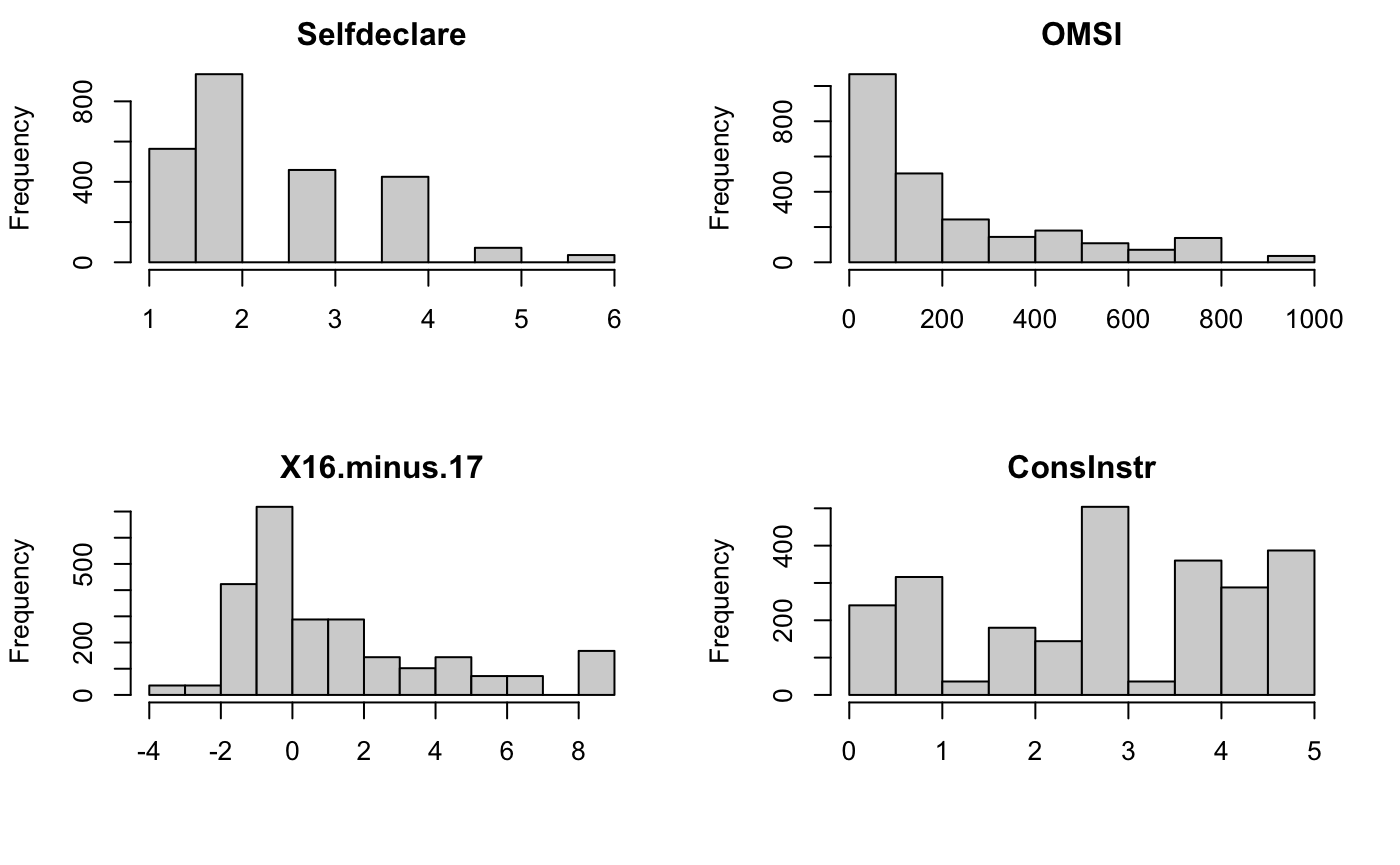
\includegraphics[width=\linewidth]{000024.png} 
        \vspace{4ex}
    \end{minipage}
    \begin{minipage}[b]{0.5\linewidth}
        \centering
        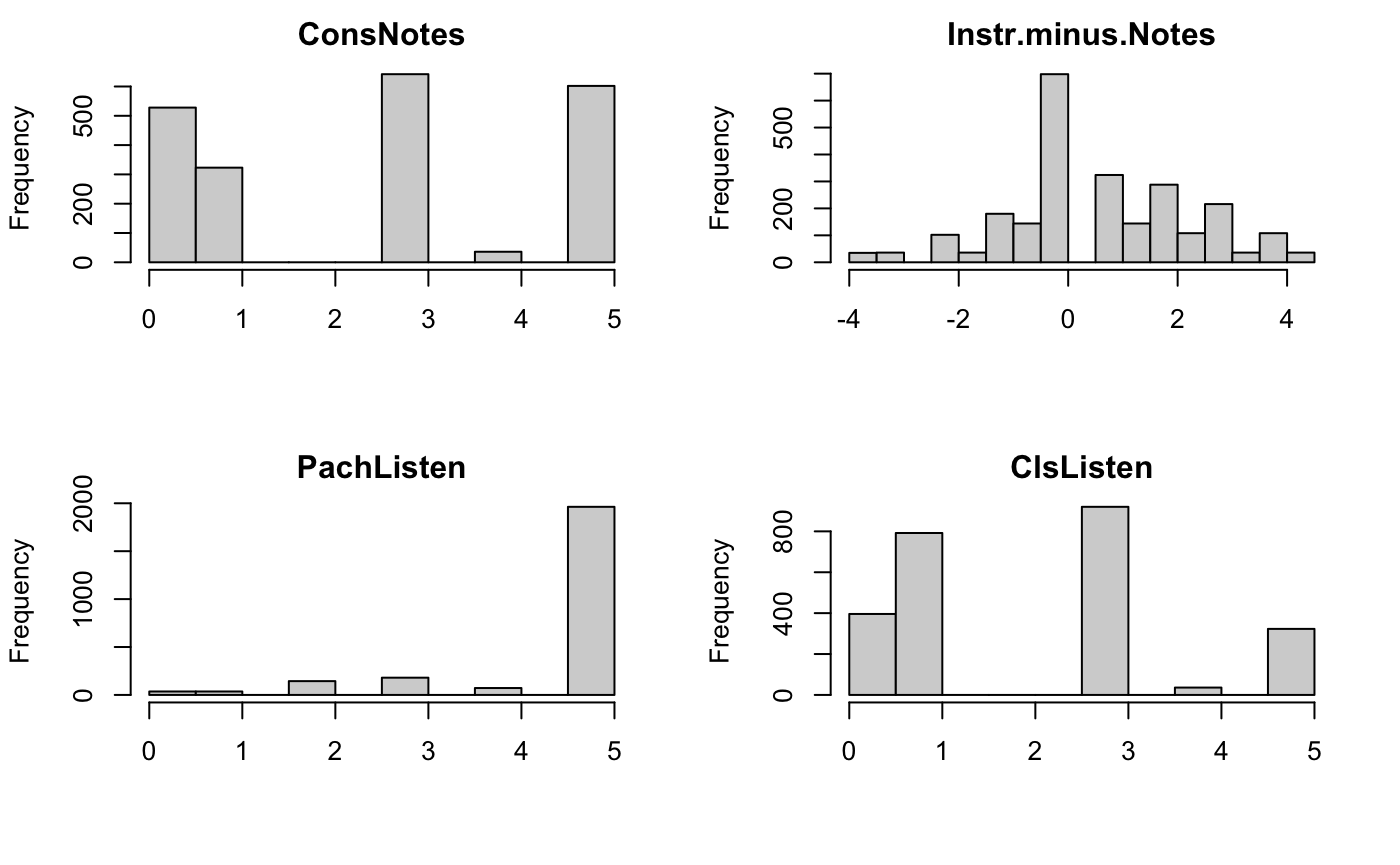
\includegraphics[width=\linewidth]{000025.png} 
        \vspace{4ex}
    \end{minipage} 
    \begin{minipage}[b]{0.5\linewidth}
        \centering
        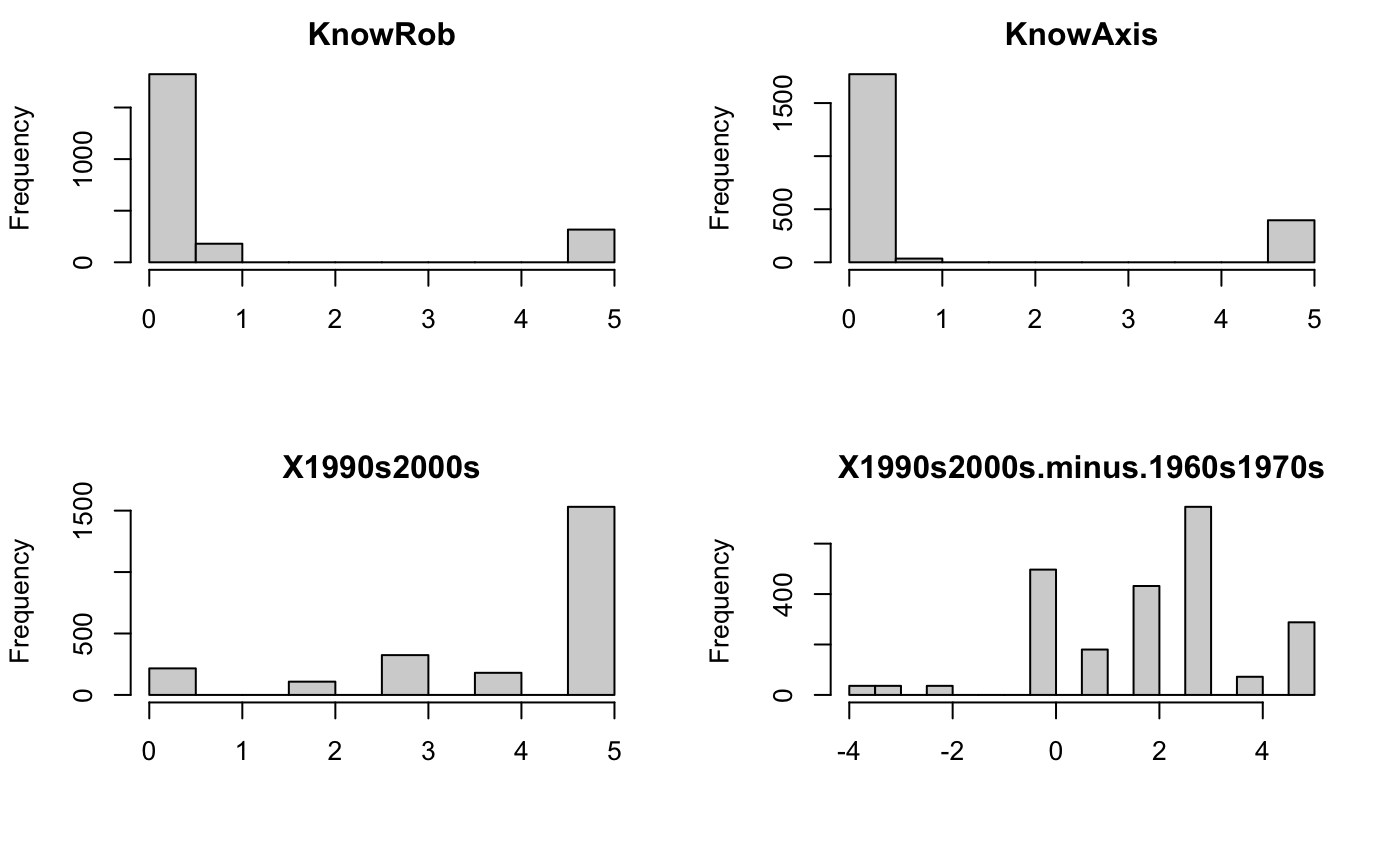
\includegraphics[width=\linewidth]{000026.png}
        \vspace{4ex}
    \end{minipage}
    \begin{minipage}[b]{0.5\linewidth}
        \centering
        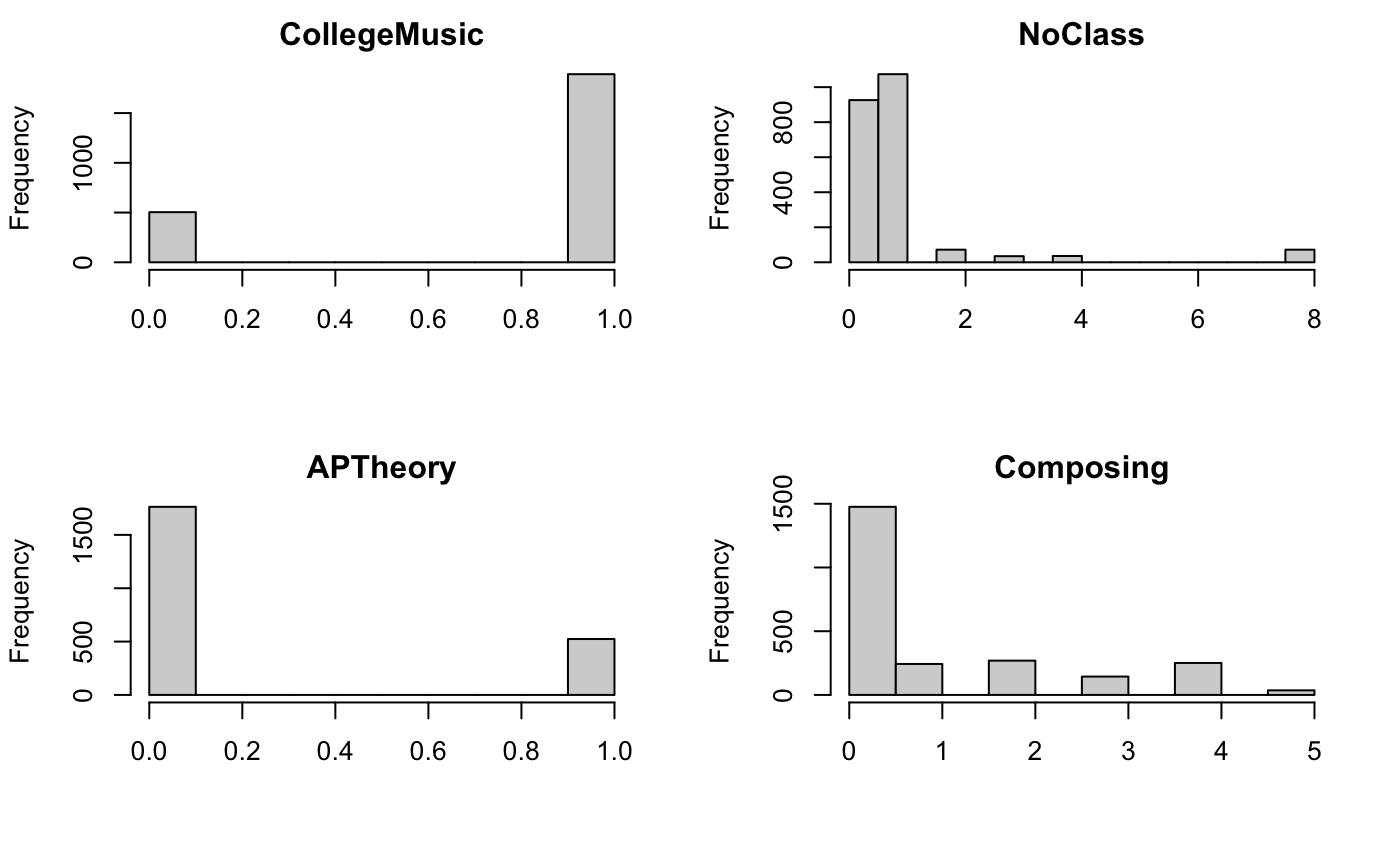
\includegraphics[width=\linewidth]{000027.png}
        \vspace{4ex}
    \end{minipage}
    \begin{minipage}[b]{0.5\linewidth}
        \centering
        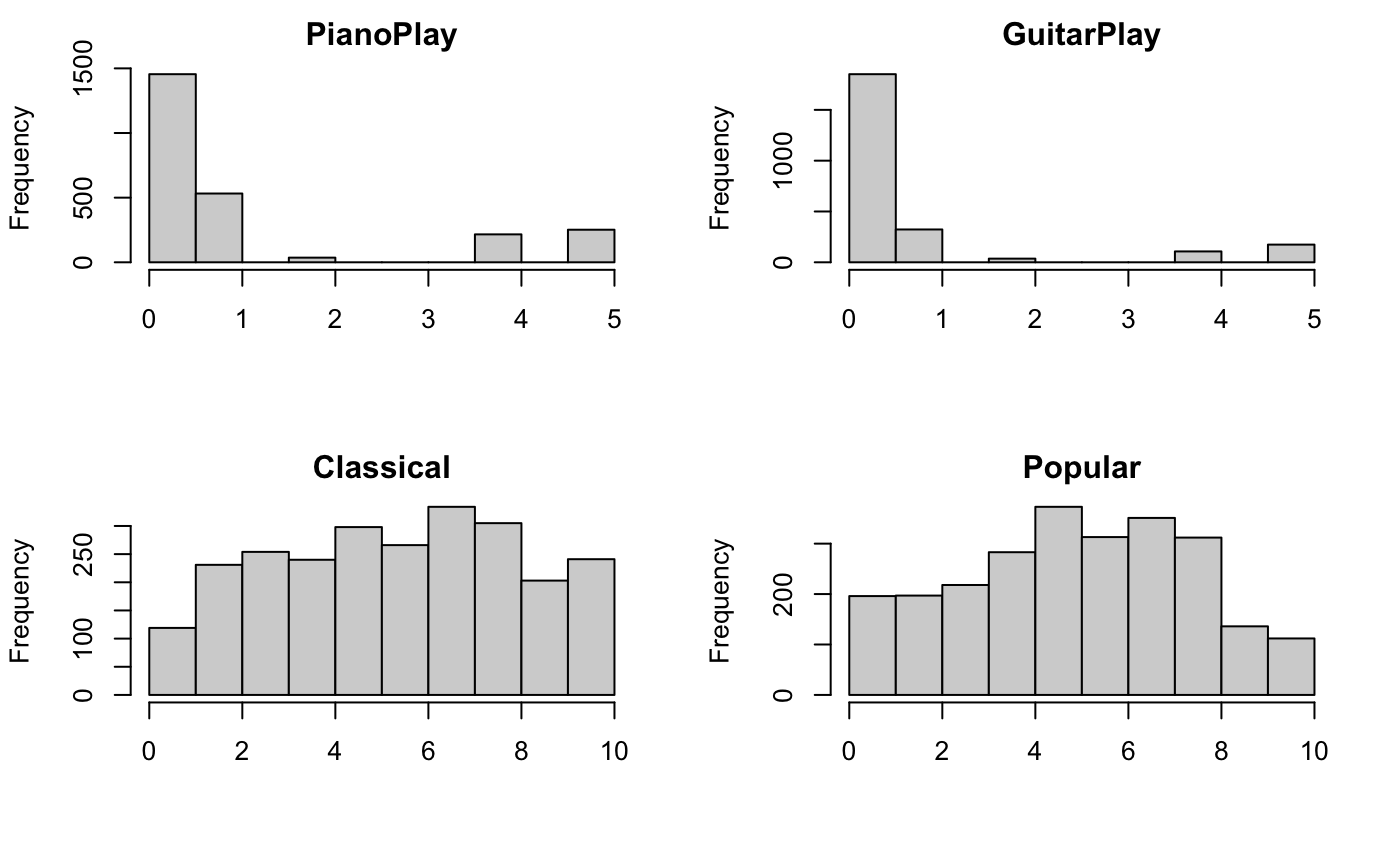
\includegraphics[width=\linewidth]{000030.png}
        \vspace{4ex}
    \end{minipage}
\end{figure}


\subsection{What experimental factor, or combinations of factors, has the strongest influence on ratings?}

To answer the first research question, model selection was conducted in four steps as mentioned in the Methods section above. Table \ref{table:models} shows the different combinations of experimental factors, interactions, and random effects that were included in each of the 17 models that were compared throughout step 1 to 3. Models 1.0 to 1.4 were compared in step one, Models 2.0 to 2.4 were compared in step two, and Models 3.1 to 3.7 were compared in step three. The final combination of design variables, interactions, and random effects selected after completing step three was used as a basis when selecting person covariates in step four of the model selection process.
\bigbreak

Table \ref{table:aicbicdic} shows the AIC, BIC, and DIC for each of the 17 models compared. Between Models 1.0 to 1.4, AIC was the lowest for Model 1.2 (model with three design variables, \texttt{Harmony}, \texttt{Instrument}, and \texttt{Voice} and interaction between \texttt{Harmony} and \texttt{Voice}) and BIC was the lowest for Model 1.1 (additive model with only three design variables). The result of the ANOVA test was that Model 1.2 was the most preferred model out of Models 1.0 and 1.4 (Appendix B.1). Between Models 2.0 to 2.4, AIC was the lowest for Model 2.2 (model with 3 design variables, interaction between \texttt{Voice} and \texttt{Harmony}, and random intercept for each participant) and BIC was the lowest for Model 2.1 (model with 3 design variables and random intercept for each participant). The result of the ANOVA test was that Model 2.2 was the most preferred model out of Models 2.0 and 2.4. For step 3, Model 2.2 was used as a basis when adding different combinations of random slope for three design variables. The correlation between the random slopes for the three design variables were forced to be zero as the random effects become more interpretable (Appendix B.3). Between Models 3.1 to 3.7, AIC and DIC were the lowest for Model 3.7 (model with 3 design variables, interaction between \texttt{Voice} and \texttt{Harmony}, random intercept for each participant, and random slopes for all three design variables), and BIC was the lowest for Model 3.4 (model with 3 design variables, interaction between \texttt{Voice} and \texttt{Harmony}, random intercept for each participant, and random slopes for \texttt{Instrument} and \texttt{Harmony}). The model chosen after completing steps 1 to 3 was Model 3.7, and the model equation can be found in Appendix B.4.

\begin{table}[!htbp]
\caption{Experimental factors, interactions, and random effects present in Models 1.0 to 1.4, Models 2.0 to 2.4, and Models 3.1 to 3.7. \label{table:models}}
\bigbreak
\centering
\begin{tabular}{|c|c|c|c|c|c|c|}
\hline
\multirow{2}{*}{\textbf{Model}} & \multirow{2}{*}{\textbf{\shortstack{3 Design \\ Variables}}} & \multirow{2}{*}{\textbf{Interactions}} & \multirow{2}{*}{\textbf{Random Intercept}} & \multicolumn{3}{c|}{\textbf{Random Slope}} \\
\cline{5-7}
 &  &  &  & Instrument & Harmony & Voice \\ 
\hline
\hline
1.0 & \xmark & \xmark & \xmark & \xmark & \xmark & \xmark \\ 
\hline
1.1 & \cmark & \xmark & \xmark & \xmark & \xmark & \xmark \\ 
\hline
1.2 & \cmark & Voice and Harmony & \xmark & \xmark & \xmark & \xmark \\ 
\hline
1.3 & \cmark & All two-way & \xmark & \xmark & \xmark & \xmark \\ 
\hline
1.4 & \cmark & All three-way & \xmark & \xmark & \xmark & \xmark \\ 
\hline
\hline
2.0 & \xmark & \xmark & \cmark & \xmark & \xmark & \xmark \\ 
\hline
2.1 & \cmark & \xmark & \cmark & \xmark & \xmark & \xmark \\ 
\hline
2.2 & \cmark & Voice and Harmony & \cmark & \xmark & \xmark & \xmark \\ 
\hline
2.3 & \cmark & All two-way & \cmark & \xmark & \xmark & \xmark \\ 
\hline
2.4 & \cmark & All three-way & \cmark & \xmark & \xmark & \xmark \\ 
\hline
\hline
3.1 & \cmark & Voice and Harmony & \cmark & \cmark & \xmark & \xmark \\ 
\hline
3.2 & \cmark & Voice and Harmony & \cmark & \xmark & \cmark & \xmark \\ 
\hline
3.3 & \cmark & Voice and Harmony & \cmark & \xmark & \xmark & \cmark \\ 
\hline
3.4 & \cmark & Voice and Harmony & \cmark & \cmark & \cmark & \xmark \\ 
\hline
3.5 & \cmark & Voice and Harmony & \cmark & \cmark & \xmark & \cmark \\ 
\hline
3.6 & \cmark & Voice and Harmony & \cmark & \xmark & \cmark & \cmark \\ 
\hline
3.7 & \cmark & Voice and Harmony & \cmark & \cmark & \cmark & \cmark \\
\hline
\end{tabular}
\end{table}


\begin{table}[!htbp]
\caption{AIC, BIC, and DIC values for Models 1, 2 and 3.\label{table:aicbicdic}}
\bigbreak
\centering
\begin{tabular}{| P{0.2\textwidth} | P{0.2\textwidth} | P{0.2\textwidth} | P{0.2\textwidth} |}
    \hline
     \textbf{Model} & \textbf{AIC} & \textbf{BIC} & \textbf{DIC} \\
     \hline
     \hline
     1.0 & 11918 & 11930 & 11918 \\
     \hline
     1.1 & 11198 & 11251 & 11198 \\
     \hline
     1.2 & 11193 & 11281 & 11193 \\
     \hline
     1.3 & 11209 & 11281 & 11209 \\
     \hline
     1.4 & 11221 & 11437 & 11221 \\
     \hline
     \hline
     2.0 & 11430 & 11448 & 11424 \\
     \hline
     2.1 & 10431 & 10489 & 10411 \\
     \hline
     2.2 & 10418 & 10511 & 10386 \\
     \hline
     2.3 & 10432 & 10583 & 10380 \\
     \hline
     2.4 & 10438 & 10659 & 10362 \\
     \hline
     \hline
     3.1 & 10044 & 10172 & 10000 \\
     \hline
     3.2 & 10334 & 10485 & 10282 \\
     \hline
     3.3 & 10430 & 10558 & 10386 \\
     \hline
     3.4 & 9902 & \cellcolor{yellow}10089 & 9838 \\
     \hline
     3.5 & 10056 & 10219 & 10000 \\
     \hline
     3.6 & 10346 & 10532 & 10282 \\
     \hline
     3.7 & \cellcolor{yellow}9901 & 10122 & \cellcolor{yellow}9825 \\
     \hline
\end{tabular}
\end{table}


\newpage
\singlespacing % single space longtable
\begin{center}
\begin{longtable}{l D{)}{)}{9)0}}
\caption{Model after selection of person covariates}
\label{table:pers-cov}
\hline
 & \multicolumn{1}{c}{Additive Fixed Effects} \\
\midrule
\endfirsthead
\toprule
 & \multicolumn{1}{c}{Additive Fixed Effects} \\
\midrule
\endhead
\bottomrule
\endfoot
\bottomrule
\endlastfoot \\
(Intercept)                                      & 4.95 \; (0.93)  \\
HarmonyI-V-IV                                    & 0.21 \; (0.20)  \\
HarmonyI-V-VI                                    & 1.27 \; (0.28)  \\
HarmonyIV-I-V                                    & -0.30 \; (0.20) \\
Instrumentpiano                                  & 1.65 \; (0.24)  \\
Instrumentstring                                 & 3.59 \; (0.31)  \\
Voicepar3rd                                      & -0.31 \; (0.20) \\
Voicepar5th                                      & -0.20 \; (0.20) \\
X16.minus.17                                     & -0.15 \; (0.05) \\
ConsNotes                                        & -0.35 \; (0.07) \\
PachListen3                                      & -1.80 \; (0.66) \\
PachListen4                                      & 1.56 \; (0.93)  \\
PachListen5                                      & -0.95 \; (0.52) \\
ClsListen1                                       & -0.28 \; (0.35) \\
ClsListen3                                       & 0.38 \; (0.42)  \\
ClsListen4                                       & 6.25 \; (1.10)  \\
ClsListen5                                       & -0.06 \; (0.54) \\
KnowRob1                                         & -0.54 \; (0.48) \\
KnowRob5                                         & 1.34 \; (0.43)  \\
KnowAxis1                                        & -6.05 \; (1.37) \\
KnowAxis5                                        & -0.47 \; (0.33) \\
X1990s2000s                                      & -0.15 \; (0.12) \\
X1990s2000s.minus.1960s1970s                     & 0.25 \; (0.09)  \\
NoClass                                          & 0.67 \; (0.18)  \\
APTheory1                                        & 2.61 \; (0.38)  \\
Composing1                                       & -0.47 \; (0.31) \\
Composing2                                       & 1.01 \; (0.48)  \\
Composing3                                       & 0.41 \; (0.43)  \\
Composing4                                       & 0.79 \; (0.55)  \\
Composing5                                       & -1.84 \; (1.24) \\
GuitarPlay1                                      & 0.43 \; (0.60)  \\
GuitarPlay2                                      & 3.48 \; (0.56)  \\
GuitarPlay4                                      & 2.23 \; (0.99)  \\
GuitarPlay5                                      & -4.50 \; (0.76) \\
HarmonyI-V-IV:Voicepar3rd                        & -0.42 \; (0.28) \\
HarmonyI-V-VI:Voicepar3rd                        & -0.71 \; (0.28) \\
HarmonyIV-I-V:Voicepar3rd                        & 0.75 \; (0.28)  \\
HarmonyI-V-IV:Voicepar5th                        & -0.21 \; (0.28) \\
HarmonyI-V-VI:Voicepar5th                        & -0.53 \; (0.28) \\
HarmonyIV-I-V:Voicepar5th                        & 0.33 \; (0.28)  \\
\midrule
AIC                                              & 6200.94         \\
BIC                                              & 6542.67         \\
Log Likelihood                                   & -3036.47        \\
Num. obs.                                        & 1540            \\
Num. groups: Subject                             & 43              \\
Var: Subject (Intercept)                         & 0.00            \\
Var: Subject.1 Instrumentguitar                  & 0.81            \\
Var: Subject.1 Instrumentpiano                   & 1.98            \\
Var: Subject.1 Instrumentstring                  & 1.35            \\
Cov: Subject.1 Instrumentguitar Instrumentpiano  & 0.42            \\
Cov: Subject.1 Instrumentguitar Instrumentstring & -0.81           \\
Cov: Subject.1 Instrumentpiano Instrumentstring  & 0.48            \\
Var: Subject.2 Voicecontrary                     & 0.00            \\
Var: Subject.2 Voicepar3rd                       & 0.12            \\
Var: Subject.2 Voicepar5th                       & 0.04            \\
Cov: Subject.2 Voicecontrary Voicepar3rd         & 0.00            \\
Cov: Subject.2 Voicecontrary Voicepar5th         & 0.00            \\
Cov: Subject.2 Voicepar3rd Voicepar5th           & 0.07            \\
Var: Subject.3 HarmonyI-IV-V                     & 0.00            \\
Var: Subject.3 HarmonyI-V-IV                     & 0.13            \\
Var: Subject.3 HarmonyI-V-VI                     & 1.68            \\
Var: Subject.3 HarmonyIV-I-V                     & 0.04            \\
Cov: Subject.3 HarmonyI-IV-V HarmonyI-V-IV       & 0.00            \\
Cov: Subject.3 HarmonyI-IV-V HarmonyI-V-VI       & 0.00            \\
Cov: Subject.3 HarmonyI-IV-V HarmonyIV-I-V       & 0.00            \\
Cov: Subject.3 HarmonyI-V-IV HarmonyI-V-VI       & 0.16            \\
Cov: Subject.3 HarmonyI-V-IV HarmonyIV-I-V       & -0.05           \\
Cov: Subject.3 HarmonyI-V-VI HarmonyIV-I-V       & 0.09            \\
Var: Residual                                    & 2.44            \\
\end{longtable}
\end{center}


\newpage
\doublespacing
In addition to the three design variables, interaction between Voice and Harmony, random intercept for each participant and three random slopes for the three design variables for each participant (Model 3.7), 12 additional person covariates were selected by two passes of backwards selection of fixed effects using AIC and BIC by \texttt{fitLMER.fnc} in step 4 of model selection (Appendix C.1). Random effects selection using DIC resulted in all three random slopes for the three design variables being kept in the model (Appendix C.2). The residual plots for the final model showed that our model seems to satisfy the assumptions of normality and constant variance of both level-1 and level-2 residuals well (Appendix C.3). Seven fixed effects have variance inflation factor (VIF) greater than 10, which is a common threshold for serious collinearity between predictors in the model \parencite[]{lecture-07}. The coefficient estimates for the fixed effects with their standard error, the coefficient estimates for random effects with their variances and covariances for the final model are shown in Table \ref{table:pers-cov}. Out of all three design variables and 12 person covariates in the model, all predictors have statistically significant levels except for the variable \texttt{X1990s2000s}. Intrepretation of all fixed effects can be found in Appendix C.4.
\bigbreak

Based on the results presented in Table \ref{table:pers-cov}, we can answer the first research question, ``What experimental factor, or combinations of factors, has the strongest influence on ratings?'' which consist of three sub-questions:


\begin{itemize}
    \item \textbf{Does Instrument exert the strongest influence among the three design factors (Instrument, Harmonic Motion, Voice Leading), as the researchers suspect?} Yes, listeners think piano and especially strings, sound more classical than guitar. The instrument ``piano'' tends to add more than 1.65 points to the Classical rating compared to the baseline instrument guitar. The instrument ``string'' tends to add more than 3.5 points to the Classical rating compared to guitar.
    \item \textbf{Among the levels of Harmonic Motion does I-V-VI have a strong association (the strongest) with classical ratings? Does it seem to matter whether the respondent is familiar with one or the other (or both) of the Pachelbel rants/comedy bits?} The harmony I-V-VI has the strongest association out of the four harmonic motions with Classical rating because it tends to add nearly one point on average to the Classical rating compared to the baseline harmony I-IV-V and adds the most to classical ratings compared to other two harmonies. Relative to baseline category 0 (``not at all''),  listeners who express modest familiarity with the Rob Paravonian's Pachelbel Rant have lower Classical ratings by about 0.5 points, whereas those with modest familiarity with the Axis of Awesome bit, reduce their classical ratings by more than six points. The giant jump ($\hat\beta_{KnowAxis=1}-6.05$) may be mainly a small-sample bias issue, since only one listener scored in category 1 on this variable (Appendix C.4) Having the highest familiarity with Pachelbel Rant adds 1.3 points to the Classical rating, while having the highest familiarity with the Axis of Awesome bit reduces Classical rating by about 0.5 points.
    \item \textbf{Among the levels of Voice Leading, does contrary motion have a strong (the strongest) association with classical ratings?} Yes, contrary motion have the strongest association with Classical rating among the levels of Voice Leading. Compared to contrary motion, having the Voice Leading pattern ``parallel 3rds'' tends to reduce Classical rating by 0.3 points. Compared to contrary motion, having the voice-leading pattern ``parallel 5ths'' tends to reduce Classical rating by 0.2 points.
\end{itemize}


\subsection{Are there differences in the way that musicians and non-musicians identify classical music?}

A new dichotomized variable called \texttt{Musician} was created by dichotomizing \texttt{Selfdeclare} variable. Statistical significance of the interaction term between \texttt{Musician} and other predictors were analyzed. In other words, \texttt{Musician} variable was 0 if the value of \texttt{Selfdeclare} was less than a certain threshold, $c$, where $c$ is a value between 1 and 6 corresponding to the levels of the \texttt{Selfdeclare} variable.

\[
     Musician_i = \left\{\begin{array}{rl}
                  0, & \mbox{\it if $Selfdeclare\leq c$}\\
                  1, & \mbox{\it otherwise}
                  \end{array}\right.
\]

Dichotomizing \texttt{Selfdeclare} variable so that about half the participants are categorized as self-declared musicians and creating a new dummy variable called \texttt{Musician} produced significant interaction between the \texttt{Musician} variable and Harmony (Appendix D). The significant interaction only involved one level of Harmony, which was I-V-VI. There are some coefficient estimates at the order of 100 or 1000 and many interactions are dropped. This means that Musicians tend to rate certain harmony structures as classical differently from how non-musicians rate them. The interactions with Musician change depending on where we dichotomize the \texttt{Selfdeclare} variable. Appendix D shows that:

\begin{itemize}
    \item Dichotomizing between 1 and 2 ($c=1$) produced no significant interaction between \texttt{Musician} variable and other predictors.
    \item Dichotomizing between 2 and 3 ($c=2$) produced significant interaction between \texttt{Musician} and \texttt{Harmony}, with $\hat{\beta}_{HarmonyI-V-VI:Musician} = 1.26$.
    \item Dichotomizing between 3 and 4 ($c=3$) produced significant interaction between \texttt{Musician} and \texttt{Harmony}, and \texttt{Musician} and \texttt{OMSI}, with $\hat{\beta}_{HarmonyI-V-VI:Musician} = 1.41$ and $\hat{\beta}_{OMSI:Musician} = -0.03$.
    \item Dichotomizing between 4 and 5 ($c=4$) produced significant interaction between \texttt{Musician} and \texttt{Harmony} with $\hat{\beta}_{HarmonyI-V-VI:Musician} = 1.95$.
    \item Dichotomizing between 5 and 6 ($c=5$) produced no significant interaction between \texttt{Musician} variable and other predictors.
\end{itemize}

Therefore, the presence or absence of interactions of the dichotomized ``Musician'' variable with design variables or with other person covariates depends strongly on the value of $c$ in the above equation. A final determination of the question of interactions of a dichotomized version of the \texttt{Selfdeclare} with design factors and other terms in the model should be determined after a discussion with the client.

\section{Discussion}

% TBD. The discussion section should move to the results section. Notice that the results section should do a brief summary of what you find in the results section. You should not do the main analysis in the discussion section. The content right now seems suitable for the result section. In future work, you need to shorten the main analysis of what you get in the results section. Also, you should mention the weakness of your analysis and mention what you can do in the future.

% Once again, the structure of the section is great. It is very easy to find the research question and then the answer. My only comment is: the discussion feels a bit methods heavy. It seems like you are narrating the process of finding the answer, whereas I think the bulk of the discussion should be implications of the results and what they mean. I also like how you are planning to address strengths and weaknesses of the dataset as well as future research and unanswered questions. Overall, very strong section.

In this report, I analyzed the influence of different experimental factors and random effects on listeners' identification of music as ``classical''.

\subsection{The influence of the three main experimental factors (Instrument, Harmony \& Voice)}

Choice of instrument seems to have an impact on listeners' identification of music as ``classical''. Listeners tend to think that piano and especially strings sound more classical than guitar. Piano and strings add about 1.65 and 3.5 points to the Classical rating, respectively, compared to musical stimuli with guitar as the instrument. Among the levels of Harmonic Motion, the harmonic motion I-V-VI has the strongest association with increasing classical rating out of the four harmonic motions tested. Compared to the baseline harmony I-IV-V, harmony I-V-VI, I-V-VI, and IV-I-V influence the classical rating by 0.2, 1.3, and -0.3 points on average, respectively. Among the levels of Voice Leading, contrary motion have the strongest association with increasing classical ratings. Compared to contrary motion, having the voice leading patterns ``parallel 3rds'' and ``parallel 5ths'' tend to reduce Classical rating by 0.3 and 0.2 points on average, respectively.

\subsection{Differences in the way that musicians and non-musicians identify classical music}

There seems to be a difference in a way that musicians and non-musicians identify classical music, but the result is sensitive to where the dichotomization of participants into musicians and non-musicians occur. If the dichotomizations of participants based on self-declaration to the question to the question ``Are you a musician'' occur on ratings between 2 to 3, 3 to 4, and 4 to 5, then there seems to be a difference in how musicians and non-musicians perceive harmonic motion I-V-VI as classical. In particular, musicians seem to think that the harmonic motion I-V-VI are more classical, adding over 1 points to classical rating. If the dichotomizations occur on ratings between 1 and 2, and 5 and 6, there seems to be no difference in how musicians and non-musicians perceive harmonic motion.

\subsection{Strengths and Weaknesses}
% Strengths
One of the strengths of this study is that the study design was well balanced across experimental conditions and subjects even after deletion of incomplete observations. Another strength of this study is that we explored many experimental factors and person covariates that could influence participants' classification of music as classical. One of the weaknesses of this study is that there are many missing data. Only 61\% of the observations were complete, and the number of subjects represented were reduced from 70 to 43 subjects after removing incomplete observations. Another weakness of the study is that the coefficient estimates of the final multi-level model may have been impacted by small-sample bias as some of the levels of the categorical variables involved only one or two participants.

\subsection{Future works}
In the future, verifying that the results are replicable in different groups of listeners would be necessary. The participants were all sampled from the undergraduate student population at the University of Pittsburgh, and there might have been hidden confounders unique to the group selected that influenced Classical ratings. Also, investigating the interaction among person covariates could be a possibility for a future work. Only the interaction between the person covariates and the Musician variable was examined in this study, but other interactions between person covariates might be influential to Classical rating. Finally, it would be interesting to repeat the analysis for Popular rating as the response variable, and compare the results to see which experimental factors influence the classification of music as ``classical'' or ``popular''.


\newpage

% REFERENCES
\printbibliography


\iffalse
\begin{hangparas}{.25in}{1}
Junker, B. (2022a), \textit{Homework 9}. Assignment sheet, 36-617 Applied Linear Regression, Nov 11, 2022. Department of Statistics and Data Science, Carnegie Mellon University.

Junker, B. (2022b), Personal Communication, November 14, 2022.

Junker, B, (2022c), \textit{Estimation and Model Selection}. Lecture notes, 36-617 Applied Linear Regression, Nov 16, 2022. Department of Statistics and Data Science, Carnegie Mellon University.

R Core Team (2017), \textit{R: A language and environment for statistical computing}. R Foundation for Statistical Computing, Vienna, Austria. URL https://www.R-project.org/.

RStudio Team (2020), \textit{R Studio: Integrated Development Environment for R}. RStudio, PBC, Boston MA. URL http://www.rstudio.com/.

Sheather, S.J. (2009), \textit{A Modern Approach to Regression with R}. New York: Springer Science + Business Media LLC.
\end{hangparas}
\fi

\end{document}

